\documentclass{standalone}

\usepackage[latin1]{inputenc}
\usepackage{amsmath}
\usepackage{amssymb}
\usepackage{amsthm}

\usepackage{tikz}
\usetikzlibrary{snakes}

%% generates a tightly fitting border around the work
%\usepackage[active,tightpage]{preview}
%\PreviewEnvironment{tikzpicture}
%\setlength\PreviewBorder{0.5mm}
%%\renewcommand\PreviewBbAdjust{-\PreviewBorder 1mm -1.15mm -0.85mm}

\usepackage{color}

%\pagestyle{empty}

\begin{document}

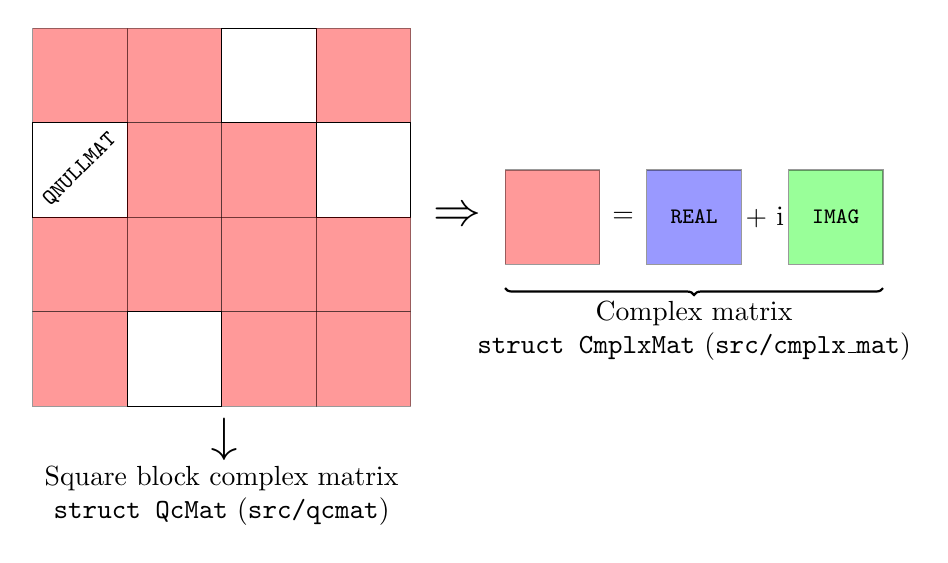
\begin{tikzpicture}[scale=0.6]
  \draw[fill=red,opacity=0.4] (6,10) rectangle ++(2,2);
  \draw[fill=red,opacity=0.4] (8,10) rectangle ++(2,2);
  \draw (6,8) rectangle ++(2,2);
  \node[rotate=45] at (7,9) {\footnotesize\texttt{QNULLMAT}};
  \draw[fill=red,opacity=0.4] (8,8) rectangle ++(2,2);
  \draw (10,10) rectangle ++(2,2);
  \draw[fill=red,opacity=0.4] (12,10) rectangle ++(2,2);
  \draw[fill=red,opacity=0.4] (10,8) rectangle ++(2,2);
  \draw (12,8) rectangle ++(2,2);
  \draw[fill=red,opacity=0.4] (6,6) rectangle ++(2,2);
  \draw[fill=red,opacity=0.4] (8,6) rectangle ++(2,2);
  \draw[fill=red,opacity=0.4] (6,4) rectangle ++(2,2);
  \draw (8,4) rectangle ++(2,2);
  \draw[fill=red,opacity=0.4] (10,6) rectangle ++(2,2);
  \draw[fill=red,opacity=0.4] (12,6) rectangle ++(2,2);
  \draw[fill=red,opacity=0.4] (10,4) rectangle ++(2,2);
  \draw[fill=red,opacity=0.4] (12,4) rectangle ++(2,2);
  \node[rotate=270] at (10,3.3) {\LARGE$\rightarrow$};
  \node[align=center] at (10,2.1) {Square block complex matrix\\\texttt{struct QcMat} (\texttt{src/qcmat})};
  %
  \node at (15,8) {\LARGE$\Rightarrow$};
  \draw[fill=red,opacity=0.4] (16,7) rectangle ++(2,2);
  \node at (18.5,8) {$=$};
  \draw[fill=blue,opacity=0.4] (19,7) rectangle ++(2,2);
  \node at (20,8) {\footnotesize\texttt{REAL}};
  \node at (21.5,8) {$+$ i};
  \draw[fill=green,opacity=0.4] (22,7) rectangle ++(2,2);
  \node at (23,8) {\footnotesize\texttt{IMAG}};
  \draw [thick, decoration={brace, mirror}, decorate] (16,6.5)--(24,6.5);
  \node[align=center] at (20,5.6) {Complex matrix\\\texttt{struct CmplxMat} (\texttt{src/cmplx\_mat})};
\end{tikzpicture}

\end{document}
